% Copyright 2019 by Till Tantau
%
% This file may be distributed and/or modified
%
% 1. under the LaTeX Project Public License and/or
% 2. under the GNU Free Documentation License.
%
% See the file doc/generic/pgf/licenses/LICENSE for more details.


\section{Specifying Coordinates\\指定坐标}

\subsection{Overview\\概述}

A \emph{coordinate} is a position on the canvas on which your picture is drawn.
\tikzname\ uses a special syntax for specifying coordinates. Coordinates are
always put in round brackets. The general syntax is
\declare{|(|\opt{|[|\meta{options}|]|}\meta{coordinate  specification}|)|}.


\emph{坐标}是在绘图画布上的位置。\tikzname\ 使用一种特殊的语法来指定坐标。坐标总是放在圆括号中。一般的语法格式为
\declare{|(|\opt{|[|\meta{选项}|]|}\meta{坐标规范}|)|}。


The \meta{coordinate specification} specifies coordinates using one of many
different possible \emph{coordinate systems}. Examples are the Cartesian
coordinate system or polar coordinates or spherical coordinates. No matter
which coordinate system is used, in the end, a specific point on the canvas is
represented by the coordinate.

\meta{坐标规范}使用许多不同的\emph{坐标系}之一来指定坐标。例如,笛卡尔坐标系、极坐标或球面坐标。无论使用哪种坐标系,最终都会用坐标表示画布上的特定点。

There are two ways of specifying which coordinate system should be used:

有两种指定使用的坐标系的方法:
%
\begin{description}
    \item[Explicitly] You can specify the coordinate system explicitly. To do
        so, you give the name of the coordinate system at the beginning,
        followed by |cs:|, which stands for ``coordinate system'', followed by
        a specification of the coordinate using the key--value syntax. Thus,
        the general syntax for \meta{coordinate specification} in the explicit
        case is |(|\meta{coordinate system}| cs:|\meta{list of key--value pairs
        specific to the coordinate system}|)|.

        {显式} 可以显式指定坐标系。为此,在开头给出坐标系的名称,后面跟着 |cs:|,其代表``坐标系'',然后使用键-值语法来指定坐标。因此,显式情况下 \meta{坐标规范} 的一般语法为 |(|\meta{坐标系}| cs:|\meta{坐标系特定的键-值对列表}|)|。
    \item[Implicitly] The explicit specification is often too verbose when
        numerous coordinates should be given. Because of this, for the
        coordinate systems that you are likely to use often a special syntax
        is provided. \tikzname\ will notice when you use a coordinate
        specified in a special syntax and will choose the correct coordinate
        system automatically.

        {隐式} 当需要给出大量坐标时,显式指定通常太冗长。因此,对于经常使用的坐标系,提供了一种特殊的语法。当使用特殊语法指定坐标时,\tikzname\ 会自动识别并选择正确的坐标系。
\end{description}

Here is an example in which explicit the coordinate systems are specified
explicitly:

下面是一个显示显式坐标系的示例:

%
\begin{codeexample}[]
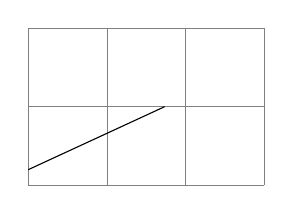
\begin{tikzpicture}
  \draw[help lines] (0,0) grid (3,2);
  \draw (canvas cs:x=0cm,y=2mm)
     -- (canvas polar cs:radius=2cm,angle=30);
\end{tikzpicture}
\end{codeexample}
%
In the next example, the coordinate systems are implicit:

在下一个示例中,坐标系是隐式指定的:

%
\begin{codeexample}[]
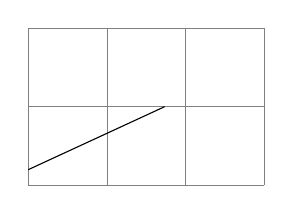
\begin{tikzpicture}
  \draw[help lines] (0,0) grid (3,2);
  \draw (0cm,2mm) -- (30:2cm);
\end{tikzpicture}
\end{codeexample}

It is possible to give options that apply only to a single coordinate, although
this makes sense for transformation options only. To give transformation
options for a single coordinate, give these options at the beginning in
brackets:

可以为单个坐标提供仅适用于变换选项的选项,尽管这仅对于变换选项有意义。要为单个坐标提供变换选项,请在方括号中的开头给出这些选项:

%
\begin{codeexample}[]
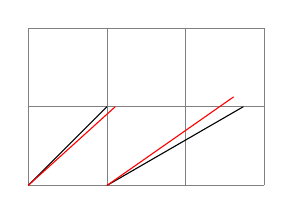
\begin{tikzpicture}
  \draw[help lines] (0,0) grid (3,2);
  \draw      (0,0) -- (1,1);
  \draw[red] (0,0) -- ([xshift=3pt] 1,1);
  \draw      (1,0) -- +(30:2cm);
  \draw[red] (1,0) -- +([shift=(135:5pt)] 30:2cm);
\end{tikzpicture}
\end{codeexample}


\subsection{Coordinate Systems\\坐标系}

